% disc.tex
\chapter{Analyse numérique}

\section{Discrétisation temporelle}

La résolution numérique des équations considérées se fait par la méthode des lignes. Il s'agit de discrétiser dans un premier temps les opérateurs spatiaux pour aboutir à une équations semi-discrétisée. Il ne reste que la dimension temporelle à considérer : il s'agit de la résolution numérique d'une équation aux dérivées ordinaires (EDO). Nous considérons ici des EDO de la forme
\begin{equation}
\dfrac{d q}{dt} = J_{\Delta} (q)
\label{eq:edo}
\end{equation}
avec la condition initiale $q(0)=q_0$. 
Ce choix de méthode est essentiellement pratique. La discrétisation spatiale et la discrétisation temporelle sont séparées, cela facilite le développement de nouvelles méthodes de discrétisations qui peuvent aisément être changées dans le code.

\subsection{Discrétisation de Runge-Kutta d'ordre 4}

Le schéma de résolution temporelle de référence que nous considérons est le schéma de Runge-Kutta d'ordre 4 (RK4). Si nous connaissons l'état de $q$ au temps $t^n = n \Delta t$ (que nous noterons $q^n$) alors nous cherchons à déterminer de façon explicite une valeur approchée de $q$ au temps $t^{n+1} = (n+1) \Delta t$. C'est à dire que nous cherchons $Q$ tel que
\begin{equation}
q^{n+1} = Q(q^n)
\end{equation}
Le schéma de Runge-Kutta d'ordre 4 est l'une des méthodes de Runge-Kutta les plus répandu, il s'écrit suivant l'algorithme \ref{alg:RK4}.

\begin{center}
\begin{minipage}[H]{12cm}
  \begin{algorithm}[H]
    \caption{: RK4}\label{alg:RK4}
    \begin{algorithmic}[1]
    \State $q^0 = q_0$ connu,
    \For{$n=0,1, \ldots$}
             \State  $K^{(1)} = J_{\Delta} \left( q^n \right)$,
             \State  $K^{(2)} = J_{\Delta} \left( q^n + \dfrac{\Delta t}{2} K^{(1)}\right)$,
             \State  $K^{(3)} = J_{\Delta} \left( q^n + \dfrac{\Delta t}{2} K^{(2)}\right)$,
             \State  $K^{(4)} = J_{\Delta} \left( q^n + \Delta t K^{(3)}\right)$,  
             \State  $q^{n+1} = q^n  + \dfrac{\Delta t}{6} \left( K^{(1)} + 2 K^{(2)} + 2 K^{(3)} + K^{(4)} \right)$.
            \EndFor
    \end{algorithmic}
    \end{algorithm}
\end{minipage}
\end{center}

On dit qu'une méthode numérique est consistante si
\begin{equation}
q^n - q(n \Delta t) = e^n
\end{equation}
et $e^n \rightarrow 0$ lors que $\Delta t \rightarrow 0$. Le schéma de Runge-Kutta d'ordre 4 est consistant à l'ordre 4. C'est à dire que l'erreur $e^n$ est de la forme
\begin{equation}
e^n = C \Delta t^4.
\end{equation}
où $C$ est indépendant de $\Delta t$. On renvoi à \cite{Demailly2016} pour preuve de consistance des méthodes de Runge-Kutta.

Il existe autres méthodes de Runge-Kutta explicites. On pensera par exemples à la méthode d'Euler Explicite ou le schéma de Heun. Il est classique de représenter une méthode de Runge-Kutta par son \textit{tableau de Butcher} :

\begin{table}[htbp]
\begin{center}
\begin{tabular}{c|c}
$b$ & $R$ \\
\hline
    & $c^T$
\end{tabular}
\end{center}
\caption{Tableau de Butcher d'une méthode de Runge-Kutta.}
\label{tab:butcher}
\end{table}

où $R$ est une matrice, $b$ et $c$ sont des vecteurs. Par exemple, le tableau de Butcher de la méthode de Runge Kutta d'ordre 4 de l'algorithme \ref{alg:RK4} est donné par :

\begin{table}[htbp]
\begin{center}
\begin{tabular}{c|cccc}
$0$   &       &      &      &      \\
$1/2$ & $1/2$ &      &      &      \\
$1/2$ & $0$   & $1/2$&      &      \\
$1$   & $0$   & $0$  & $1$  &      \\  
\hline
      & $1/6$ & $1/3$& $1/3$& $1/6$\\
\end{tabular}
\end{center}
\caption{Tableau de Butcher de la méthode de Runge Kutta d'ordre 4 (algorithme \ref{alg:RK4}).}
\end{table}
Les matrices associées au tableau de Butcher pour RK4 sont
\begin{equation}
R= \begin{bmatrix}
0 & 0 & 0 & 0 \\
1/2& 0& 0 & 0 \\
0 &1/2& 0 & 0 \\
0 & 0 & 1 & 0
\end{bmatrix}
\hspace{1cm}
b=\begin{bmatrix}
0\\1/2\\1/2\\1
\end{bmatrix}
\hspace{1cm}
c=\begin{bmatrix}
1/6\\1/3\\1/3\\1/6
\end{bmatrix}.
\end{equation}

\begin{proposition}
Une méthode de Runge-Kutta est explicite si $R$ est triangulaire inférieure strictement.
\end{proposition}




\subsection{Stabilité}

La \textit{stabilité linéaire} d'un schémas en temps est une notion essentielle associée à un schéma. Cette notion recouvre de nombreux aspects dans la littérature.
Un schéma d'intégration en temps permet de calculer $q^n$ une approximation de $q(n \Delta t)$ à une erreur $e^n$ près :
\begin{equation}
q^n = q(n \Delta t) + e^n.
\label{eq:scheme_erreur}
\end{equation}

La stabilité du schéma est essentielle. Nous distinguons deux principales notions de stabilité :
\begin{enumerate}
\item La \textit{stabilité au sens de Von Neumann} établi une relation de convergence de $q^n$ vers $q(n \Delta t)$ pour tout $1 \leq n \leq N$ lorsque $\Delta t \rightarrow 0$ et $N \rightarrow + \infty$. 
La stabilité de Von Neumann du schéma \eqref{eq:scheme_erreur} se traduit par
\begin{equation}
\exists C >0, \forall n \in \{ 0 , \cdots , N \}, \forall (N, \Delta t) \in \left\lbrace \mathbb{N} \times \mathbb{R}^+ \text{ tels que } N \Delta t = T \right\rbrace, \| q^n \| \leq C.
\end{equation}
Cette propriété traduit le fait que l'erreur doit rester uniformément bordée lorsque l'on raffine la discrétisation. La stabilité au sens de Von Neumann ne permet pas d'assurer la convergence vers la solution de l'équation différentielle lorsque l'on raffine le maillage, il s'agit là de la consistance. Si un schéma est stable et consistant, alors il y a convergence de la solution numérique vers la solution exacte sur un intervalle borné lorsque l'on raffine, il s'agit du théorème de Lax.

\item La \textit{Stabilité asymptotique} se caractérise par le compostement de la solution numérique $q^n$ sur un intervalle non borné à $\Delta t$ fixé. On distingues deux types de stabilités asymptotiques :
\begin{itemize}
\item la suite $(q^n)_{n \in \mathbb{N}}$ est bornée,
\item La suite $q^n \rightarrow 0$ lorsque $n \rightarrow + \infty$.
\end{itemize}
la stabilité asymptotique est liée à l'équation différentielle résolue. En effet si la solution exacte de l'équation résolue tend vers $0$ alors la solution numérique doit tendre vers $0$ aussi. On note cependant que la stabilité asymptotique peut n'être vérifiée que sous une contrainte sur $\Delta t$.
\end{enumerate} 

Nous nous limitons à la notion de \textit{stabilité linéaire asymptotique}, appelée stabilité linéaire. Il s'agit de la stabilité asymptotique appliquée à l'équation de Dahlquist :
\begin{equation}
\left\lbrace 
\begin{array}{rcl}
q' & = & \lambda q \\
q(0) & = & q_0.
\end{array}
\right.
\label{eq:dahlquist}
\end{equation}
avec $\lambda \in \mathbb{C}^- = \{ \lambda_1 + i \lambda_2 \text{ tels que } (\lambda_1, \lambda_2) \in \mathbb{R}^- \times \mathbb{R} \}$. La solution de cette équation est explicitement donnée par 
\begin{equation}
q(t) = e^{\lambda t} q_0
\end{equation}
On remarque immédiatement que $q$ est bornée (par $q_0$) si Re$(\lambda) \leq 0$ et $q(t) \rightarrow 0$ lorsque $t \rightarrow + \infty$ si Re$(\lambda) <0$.

\begin{proposition}
Soit une méthode de Runge-Kutta appliquée à la résolution de l'équation \eqref{eq:dahlquist}. En utilisant les notations du tableau de Butcher \ref{tab:butcher}, on a 
\begin{equation}
q^{n+1} = r(\lambda \Delta t) q^n,
\end{equation}
avec $r$ donné par 
\begin{equation}
r(\theta) = 1 + \theta c^T \cdot \left( (id - \theta R)^{-1} \mathbf{1} \right).
\end{equation}
\end{proposition}

\begin{proof}
Si l'on note $K = [K_1, K_2, ...]^T$, alors $K$ est solution de 
\begin{equation}
K = \lambda q^n +  \lambda \Delta t R K
\end{equation}
donc, $K = (id - \lambda \Delta t R)^{-1} \mathbf{1}$.
De là, il découle que 
\begin{equation}
q^{n+1} = q^n + \theta c^T \cdot \left( (id - \theta R)^{-1} q^n \right).
\end{equation} 
avec $\theta = \lambda \Delta t$. D'où le résultat.
\end{proof}
On note que si la méthode est explicite alors $R$ est nilpotente donc $r$ est polynomiale en $\theta$, 
en particulier, pour la méthode de Runge-Kutta d'ordre 4, on a 
\begin{equation}
r(\theta) = 1 + \theta + \dfrac{\theta^2}{2} + \dfrac{\theta^3}{6} + \dfrac{\theta^4}{24} 
\end{equation}
alors le résultat de stabilité est le suivant :
\begin{proposition}
La méthode de Runge-Kutta d'ordre 4 (RK4) est asymptotiquement stable pour l'équation \eqref{eq:dahlquist} si et seulement si
\begin{equation}
\vert 1 + \theta + \dfrac{\theta^2}{2} + \dfrac{\theta^3}{6} + \dfrac{\theta^4}{24}  \vert \leq 1,
\end{equation}
avec $\theta = \lambda \Delta t$.
\end{proposition}
On définit la zone de stabilité de RK4, notée $\mathcal{D}_{RK4}$, par
\begin{equation}
\mathcal{D}_{RK4} = \left\lbrace \theta \in \mathbb{C} \text{ tels que } \vert 1 + \theta + \dfrac{\theta^2}{2} + \dfrac{\theta^3}{6} + \dfrac{\theta^4}{24}  \vert \leq 1 \right\rbrace
\end{equation} 
Dans la figure \ref{fig:stab_area}, on présente les zones de stabilités de différentes méthodes de Runge-Kutta explicites.
\begin{figure}[htbp]
\begin{center}
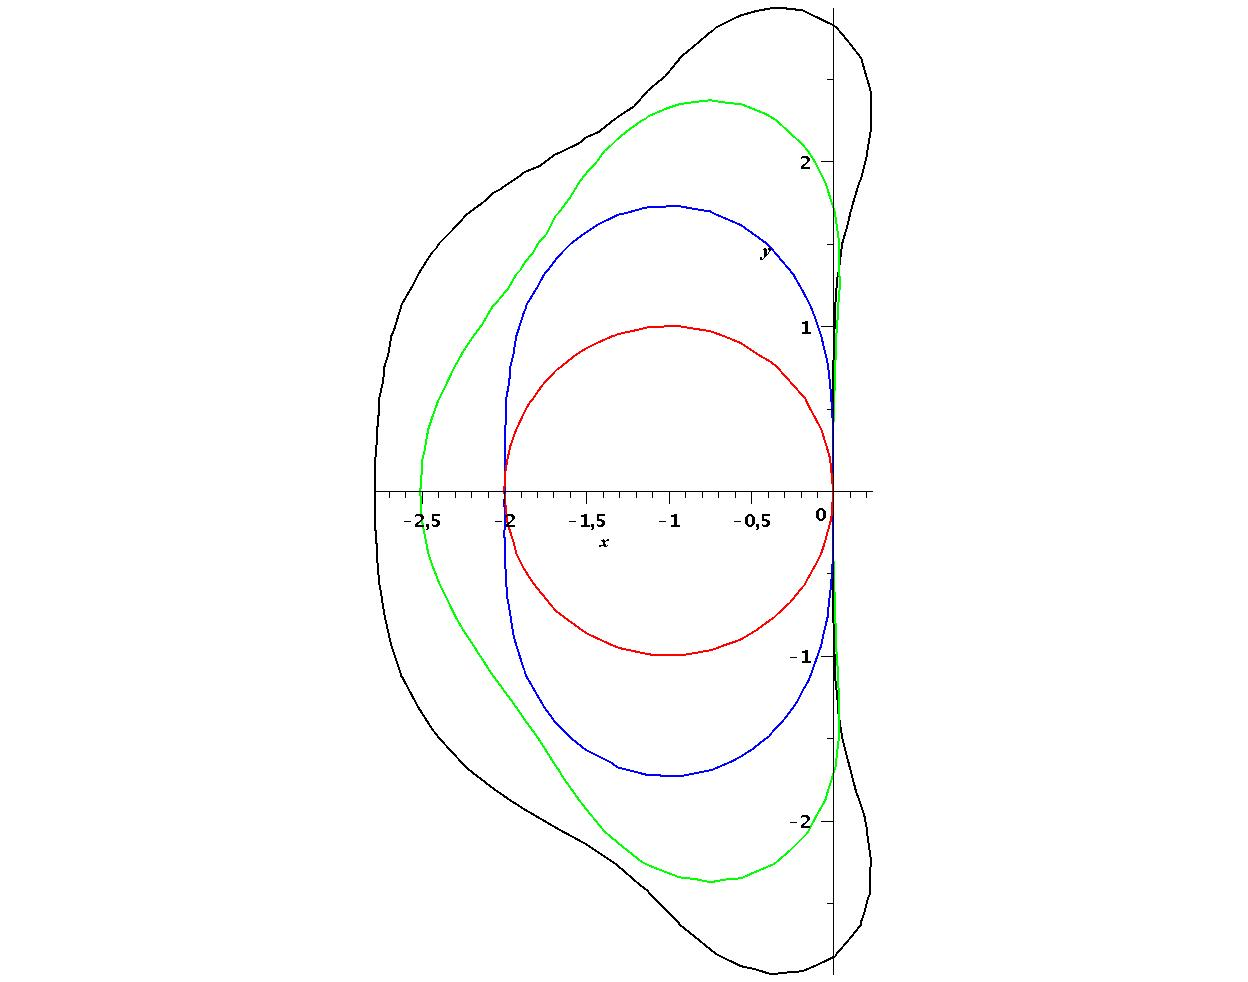
\includegraphics[scale=0.2]{stabilityarea_color.jpeg}
\end{center}
\caption{Zones de stabilités de différentes méthodes de Runge-Kutta explicites dans le plan complexe. La zone de stabilité de RK4 est délimitée par le trait noir. Les traits vert, bleu et rouge sont respectivement pour des méthodes de Runge-Kutta d'ordre 3, 2 et la méthode d'Euler Explicite.}
\label{fig:stab_area}
\end{figure}
En particulier, comme détaillé dans \cite{Hundsdorfer2013}, on note que
\begin{equation}
\mathcal{D}_{RK4} \cap i \mathbb{R} = i \left[-\sqrt{2},\sqrt{2}\right].
\end{equation}





\subsection{Schémas de Runge-Kutta pour les systèmes d'équations différentielles}

La notion de stabilité linéaire appliquée à l'équation de Dahlquist \eqref{eq:dahlquist} est étendue au système d'équations différentielles
\begin{equation}
\left\lbrace
\begin{array}{rcl}
\mathbf{q}' & = & J \mathbf{q} \\
\mathbf{q}(0) & = & \mathbf{q}_0 
\end{array}
\right.
\label{eq:dahlquist_mat}
\end{equation}
où $\mathbf{q} = \begin{bmatrix}
q_1(t) & q_2(t) & \cdots & q_N(t)
\end{bmatrix}^T \in \mathbb{R}^N$.
$q_i$ désigne une fonction de $\mathbb{R}^+$ dans $\mathbb{C}$, $J \in \mathbb{M}_N (\mathbb{C})$ désigne une matrice carré. On se restreint au cas où $J$ est une matrice diagonalisable telle que 
\begin{equation}
\text{Sp}(J) \subset \mathbb{C}^-.
\end{equation}
Cette dernière propriété permet d'assurer que la solution de \eqref{eq:dahlquist_mat} est bornée. Cette solution est donnée par 
\begin{equation}
\mathbf{q}(t) = e^{Jt}\mathbf{q}_0 \text{ avec } t \in \mathbb{R}^+.
\end{equation}
Comme $J$ est diagonalisable, il existe $P \in \mathbb{M}_N(\mathbb{R})$ une matrice de passage et $\Lambda \in \mathbb{M}_N(\mathbb{R})$ matrice diagonale (contenant les valeurs propres de $J$) tels que
\begin{equation}
J = P^{-1}\Lambda P
\end{equation}
De la, il vient que 
\begin{equation}
e^{Jt} = P^{-1}e^{\Lambda t}P,
\end{equation}
donc la solution de \eqref{eq:dahlquist_mat} vérifie l'égalité 
\begin{equation}
\mathbf{q}(t) = e^{Jt}\mathbf{q}_0 = P^{-1}e^{\Lambda t}P\mathbf{q}_0.
\end{equation}

A présent,considérons que l'équation \eqref{eq:dahlquist_mat} est discrétisée via la méthode de Runge Kutta d'ordre 4 de l'algorithme \ref{alg:RK4}. On obtient alors 
\begin{equation}
\mathbf{q}^{n+1} = r(\Delta t J) \mathbf{q}^n
\end{equation}
où $r$ est donné par 
\begin{equation}
r(\theta) = 1 + \theta + \dfrac{\theta^2}{2} + \dfrac{\theta^3}{6} + \dfrac{\theta^4}{24}.
\end{equation}
Comme $J$ est diagonalisable, on a même
\begin{equation}
\mathbf{q}^{n+1} = P^{-1}r(\Delta t \Lambda)P \mathbf{q}^n
\end{equation}
De la, on déduit la relation liant $\mathbf{q}^n$ à la condition initiale $\mathbf{q}_0$ : 
\begin{equation}
\mathbf{q}^n = r(\Delta t J) \mathbf{q}_0 = P^{-1}r(\Delta t \Lambda)P \mathbf{q}_0.
\end{equation}
Le schémas utilisé est dit linéairement stable si $\left( \| \mathbf{q}^n \| \right)_{n \in \mathbb{N}}$ est une suite bornée. Comme $J$ est diagonalisable, cela revient à dire que $| r(\Delta t \lambda) | \leq 1$ avec $\lambda \in $ Sp$(J)$.

\begin{proposition}
Le schéma d'intégration est linéairement stable si
\begin{equation}
\forall \lambda \in \text{Sp}(J), |r(\Delta t \lambda)| \leq 1.
\end{equation}
Ce qui est équivalent à dire
\begin{equation}
\text{Sp}(\Delta t J) \subset \mathcal{D}_{RK4}.
\end{equation}
Comme $r$ est un polynôme, on a même la stabilité linéaire si
\begin{equation}
\rho(r(\Delta t J)) \leq 1
\end{equation}
où $\rho$ désigne le rayon spectrale.
\end{proposition}










\section{Equation d'advection en dimension 1}

Dans cette section, on s'intéresse à l'équation de transport
\begin{equation}
\dfrac{\partial u}{\partial t} + c \dfrac{\partial u}{\partial x} = 0
\label{eq:transport_1D}
\end{equation}
pour $x \in [0,L]$, $t>0$ et avec $u(t=0,x)=u_0(x)$. On se place en contexte périodique, de période $L$. On a en particulier $u(t,0)=u(t,L)$ pour tout $t \geq 0$. $c$ est une constante positive. La solution exacte de cette équation est connue et donnée par 
\begin{proposition}
La solution de l'équation \eqref{eq:transport_1D} est donnée par 
\begin{equation}
u(t,x) = u_0(x-ct) = \gsum_{k \in \mathbb{Z}} \exp \left[ i \dfrac{2 \pi k}{L} (x-ct) \right] \hat{u}_0^k
\end{equation}
où $\hat{u}_0^k = \dfrac{1}{\sqrt{L}} \gint_0^L u_0(x) \exp \left[ - i \dfrac{2 \pi k}{L}x \right] dx$ désigne la $ki$ème transformée de Fourier de $u_0$.
\end{proposition}

\begin{proof}
La solution de \eqref{eq:transport_1D} est unique, en effet si $u_1$ et $u_2$ sont solutions (distinctes) de \eqref{eq:transport_1D} alors $w = u_1-u_2$ est une solution $L-$périodique de 
\begin{equation}
\dfrac{\partial w}{\partial t} = - \dfrac{\partial  cw}{\partial x}
\end{equation}
vérifiant $w(t=0,x)=0$ pour tout $x$. En multipliant par $w$ et en intégrant sur $[0,L]$, on obtient l'équation
\begin{equation*}
\dfrac{1}{2} \dfrac{d}{dt} \| w \|_{L^2}^2 = - \gint_{0}^L cw \dfrac{\partial w}{\partial x} = - \dfrac{c}{2} \gint_{0}^L \dfrac{\partial w^2}{\partial x} = 0 \text{ par périodicité de }w.
\end{equation*}
donc $\| w \|_{L^2}^2=\| w_{|t=0} \|_{L^2}^2 = 0$ et $w=0$, d'où l'unicité.

On peut facilement vérifier que $(t,x) \mapsto u_0(x-ct)$ et $(t,x) \mapsto \gsum_{k \in \mathbb{Z}} \exp \left[ i \dfrac{2 \pi k}{L} (x-ct) \right] \hat{u}_0^k$ sont solutions de \eqref{eq:transport_1D}. Par unicité de la solution, on obtient le résultat souhaité.
\end{proof}
Cette solution est une translation périodique de la condition initiale. Dans cette section, nous comparons la solution théorique de \eqref{eq:transport_1D} avec une solution numérique obtenue à l'aide de différents opérateurs ou outils de discrétisations évoqués dans les parties précédentes.









\subsection{Discrétisation}

La discrétisation est effectuée en utilisant la méthode des lignes. Dans un premier temps, il s'agit de discrétiser les opérateurs spatiaux. On aboutit à une EDO que nous résolvons par une méthode de Runge-Kutta. Nous utilisons dans cette partie les notations de la section \ref{sec:notation_1D}.
 
On a vu dans les parties précédentes que $\delta_x^H u^*$ était une bonne approximation de $\partial_x u^*$. On remplace l'opérateur de dérivation spatiale $\partial_x$ par l'opérateur de dérivation hermitien $\delta_x^H$.
On cherche alors $\mathfrak{u}$ approximation de $u^*$ aux points du maillage et solution de 
\begin{equation}
\left\lbrace
\begin{array}{rcl}
\dfrac{d \mathfrak{u}}{dt} & = & - c \delta_x^H \mathfrak{u} \\
\mathfrak{u}_{|t=0} & = & u_0^*
\end{array}
\right.
\end{equation}
Si l'on note matriciellement 
\begin{equation}
U = \begin{bmatrix}
\mathfrak{u}_1 \\
\mathfrak{u}_2 \\
\vdots \\
\mathfrak{u}_N
\end{bmatrix} \in \mathbb{R}^N \text{ et } U_0 = \begin{bmatrix}
u_0(x_1) \\
u_0(x_2) \\
\vdots \\
u_0(x_N)
\end{bmatrix} \in \mathbb{R}^N
\end{equation}
les vecteurs contenant les composantes de $\mathfrak{u}$ (chaque composante est dépendante de $t$) et de $u_0^*$, alors $U$ est solution du système d'équations différentielles :
\begin{equation}
\left\lbrace
\begin{array}{rcl}
\dfrac{d U}{dt} & = & - c P^{-1}K U \\
U_{|t=0} & = & U_0
\end{array}
\right. .
\end{equation}
La solution d'un tel système est donnée par 
\begin{equation}
U(t) = \exp\left[ - c P^{-1}K t\right] U_0.
\end{equation}

On a déjà vu dans la proposition \ref{prop:eigen_mat_hermitien} que $P^{-1}K$ est une matrice de $\mathbb{M}_N(\mathbb{R})$ qui admet $N$ valeur propres distinctes. $P^{-1}K$ est diagonalisable, il existe $V$ une matrice de passage et $\Lambda$ une matrice diagonale tels que 
\begin{equation}
P^{-1}K = V^T \Lambda V.
\end{equation}
Ces matrices sont données par 
\begin{equation}
\Lambda = \begin{bmatrix}
\omega^1 &   &   &   &   \\ 
  & \omega^2 &   & (0) &   \\ 
  &   & \ddots &   &   \\ 
  & (0) &   & \omega^{N-1} &   \\ 
  &   &   &   & \omega^N
\end{bmatrix} \text{ et }
V = \begin{bmatrix}
  &   &   &   &   \\ 
\vdots & \vdots  &   & \vdots  & \vdots  \\ 
U^1 & U^2 & \cdots & U^{N-1} & U^N \\ 
\vdots &\vdots &  &\vdots &\vdots \\ 
  &   &   &   &  
\end{bmatrix} 
\end{equation}
avec les vecteurs propres $U^k$ vérifiant
\begin{equation}
U^k = \begin{bmatrix}
\mathfrak{u}^k_1\\
\mathfrak{u}^k_2\\
\vdots \\
\mathfrak{u}^k_N\\
\end{bmatrix}
\end{equation} 
et les valeurs propres associées $\omega^k$. Les valeurs de $\omega^k$ et $\mathfrak{u}^k_j$ sont données par la proposition \ref{prop:vp_herm}. On déduit directement de ces égalités que 
\begin{equation}
U(t) = V^T \exp \left[-c \Lambda t \right] V U_0
\end{equation}
d'où la solution approchée de \eqref{eq:transport_1D} discrétisée en espace et évaluée en $x_j$ est donnée par 
\begin{equation}
u(t,x_m) \approx \mathfrak{u}_j(t) = \dfrac{1}{N} \gsum_{k=1}^N \gsum_{j=1}^N  \exp \left[ i l \left( k + j \right) \dfrac{2 \pi}{N} \right] \exp \left[ - c \omega^j \right] u_0(x_p)
\end{equation}


\subsection{Stabilité}

\subsection{Relations de conservations}




\section{Equation des ondes}

\subsection{Discrétisation}

\subsection{Consistance et Stabilité}

\subsection{Relations de conservations}